Introduction and motivation with 8 TeV cross section and rate
\section{Event Selection}
\label{sec:RA2_sel}

\subsection{Data samples and trigger}
\label{subsec:RA2_samples_trigger}

\subsection{Event Cleaning}
\label{subsec:RA2_cleaning}

\subsection{Baseline Selection}
\label{subsec:RA2_baseline}

\subsection{Exclusive Search Regions}
\label{subsec:RA2_search_regions}

\section{QCD Background Estimation with the Rebalance-And-Smear Method}
\label{subsec:RA2_QCD}

\subsection{Rebalance Procedure using Kinematic Fits}
\label{subsec:RA2_reb}

\subsection{Response Smearing}
\label{subsec:RA2_smear}

\subsection{Validation Tests}
\label{subsec:RA2_clsoure}

\subsection{Systematic Uncertainties}
\label{subsec:RA2_syst_unc}

\subsection{QCD Background Prediction}
\label{subsec:RA2_qcd_pred}

\section{Estimation of Non-QCD Backgrounds}
\label{sec:RA2_Non-QCD}

\subsection{Invisible Z Background}
\label{subsec:RA2_Zinv}

\subsection{Hadronic $\tau$ Background}
\label{subsec:RA2_tauhad}

\subsection{Lost-Lepton Background}
\label{subsec:RA2_lostlepton}

\section{Results and Interpretation}
\label{sec:RA2_results}

\subsection{Comparison to Other Measurements}
\label{subsec:RA2_comp}

\begin{figure}[!tp]
  \centering
  \begin{tabular}{c}
    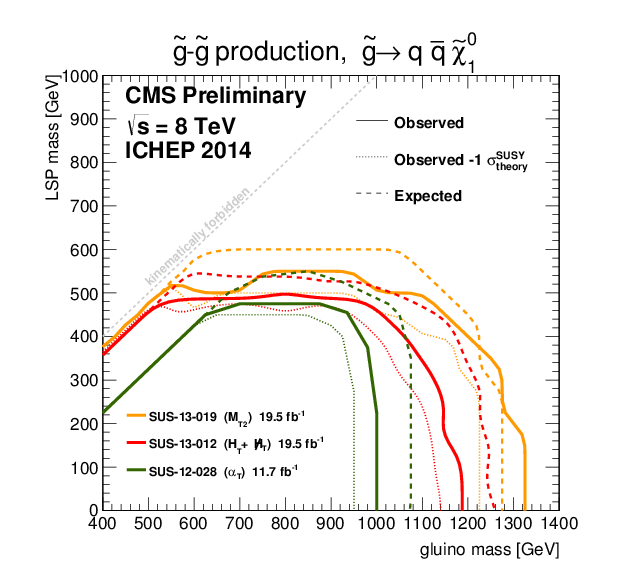
\includegraphics[width=0.9\textwidth]{figures/T1_ICHEP2014_All.png}
  \end{tabular}
  \caption{Comparison of various exclusion limits derived by different CMS anlayses for the SMS T1qqqq. Taken from ... (cms susy public results).}
  \label{fig:T1_comp}
\end{figure}

\begin{figure}[!tp]
  \centering
  \begin{tabular}{c}
    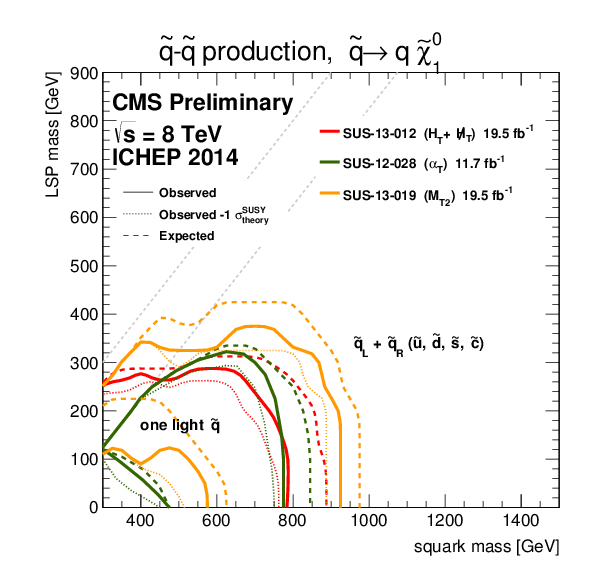
\includegraphics[width=0.9\textwidth]{figures/T2_ICHEP2014.png}
  \end{tabular}
  \caption{Comparison of various exclusion limits derived by different CMS anlayses for the SMS T2qq. Taken from ... (cms susy public results).}
  \label{fig:T1_comp}
\end{figure}

\begin{figure}[!tp]
  \centering
  \begin{tabular}{c}
    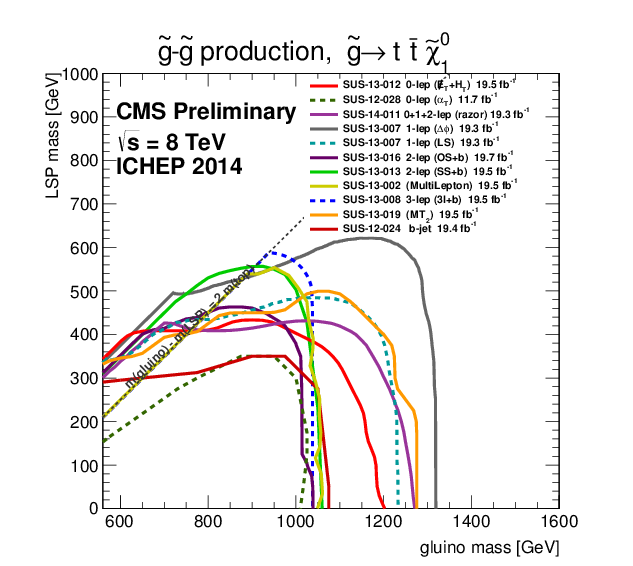
\includegraphics[width=0.9\textwidth]{figures/T1tttt_ICHEP2014_All.png}
  \end{tabular}
  \caption{Comparison of various exclusion limits derived by different CMS anlayses for the SMS T1tttt. Taken from ... (cms susy public results).}
  \label{fig:T1_comp}
\end{figure}

\section{Status of natural supersymmetry after LHC Run-I}
\label{sec:susy_status}


